\chapter{Trabajando con VMs en oVirt}
\label{ch:trabajando}

\section{Barra de herramientas}
\label{sec:controles}

Si volvemos a la lista de las máquinas, veremos una lista de herramientas en la parte superior. La siguiente captura los muestra numerados, con una lista explicando su función:

\begin{figure}[ht]
  \centering
  
\includegraphics[scale=0.50]{ovirt-vms-toolbar.png}
  %\caption{\label{fig:label} Barra de herramientas}
\end{figure}

\begin{enumerate}
\item \textbf{New VM:} Crea una nueva máquina virtual. Éste botón abre el diálogo que vimos en la sección anterior.
\item \textbf{Import:} Importa una máquina virtual.
\item \textbf{Edit:} Edita las propiedades de la máquina.
\item \textbf{Remove:} Borra la máquina virtual. Por razones obvias, ésto sólo se puede hacer si la máquina está apagada.
\item \textbf{Clone VM:} Clona la máquina virtual.
\item \textbf{Run Once:} Ejecuta una única vez.
\item \textbf{Flecha verde:} Ejecuta una única vez.
\item \textbf{Luna azul:} Suspende la ejecución de la máquina.
\item \textbf{Flecha roja:} Envía señal de apagado a la máquina virtual.
\item \textbf{Reiniciar:} Envía señal de reinicio a la máquina virtual.
\item \textbf{Consola:} Accede a la consola.
\item \textbf{Migrate:} Migra la máquina virtual.
\item \textbf{Cancel Migration:} Cancela la migración en curso.
\item \textbf{Cancel Conversion:} Cancela la conversión en curso.
\item \textbf{Make Template:} Crea una plantilla a partir del estado actual de la máquina virtual.
\item \textbf{Export:} Exporta la máquina virtual.
\item \textbf{Create Snapshot:} Crea una instantánea de la máquina virtual.
\item \textbf{Refresh:} Refresca la lista de máquinas virtuales de forma manual.
\item Cambia la tasa de refresco de la lista de máquinas virtuales.
\end{enumerate}

\section{Accediendo a consola}
\label{sec:consola}

\section[Exportando / Importando]{Exportando o importando máquinas virtuales}
\label{sec:consola}

\subsection{Exportando máquinas}
\label{subsec:exportando}

Para exportar antes una máquina virtual, deberemos importar, tal y como vimos en el apartado de instalación de oVirt, otro dominio de almacenamiento más, en este caso con función \textbf{export}. Cuando esté importado y activo, podemos proceder a exportar la máquina virtual:

\begin{figure}[ht]
  \centering
  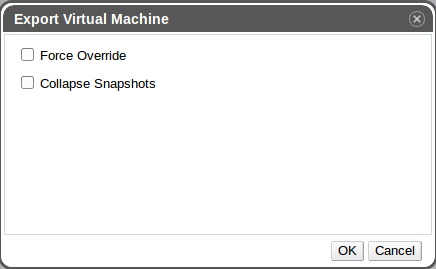
\includegraphics[scale=0.70]{ovirt-export.png}
  \caption{\label{fig:exportandovm} Exportando la máquina virtual.}
\end{figure}

Ésto servirá para poder mover una máquina virtual entre \emph{datacenters}. Es importante remarcar que un dominio export sólo puede estar activo en un clúster a la vez.

Cuando hayamos exportado la máquina a un dominio de almacenamiento, podemos comprimirlo y pasar el archivo resultantes para que otros usuarios de oVirt puedan importar el .ovf resultante a sus clústers.


\subsection{Importando máquinas}
\label{subsec:importando}

Para importar máquinas virtuales, tenemos diferentes opciones:

\begin{itemize}
\item VMware
\item \textbf{Dominio de export: } Carga las máquinas de un dominio de almacenamiento, especificado durante el proceso de exportado.
\item \textbf{Virtual Appliance (fichero OVA): } Carga las máquinas virtuales desde un fichero OVA.\@ En ésta opción sólo necesitaremos especificar la ruta absouta al fichero OVA, y el host del clúster desde el cual se va a cargar el fichero.
\end{itemize}

\begin{TMbulletin}{warning}{$¡$Cuidado!}
  La función de importado de ficheros Open Virtualization Format sólo funciona con OVFs generados por oVirt y comprimidos con gzip.
\end{TMbulletin}

La primera captura muestra la pantalla inicial de importación mediante dominio, en la cual vemos cómo se debe cargar primero el dominio, tras lo cual aparecerá la lista de máquinas virtuales del dominio, pudiendo importar una, o más máquinas.

La segunda muestra una sección con pestañas similar al \emph{overview} de las máquinas virtuales, que nos permite cambiar ciertos aspectos de la configuración de la máquina, y definir el clúster y perfil de CPU al cual se va a importar la máquina.

\begin{figure}[ht!]
  \centering
  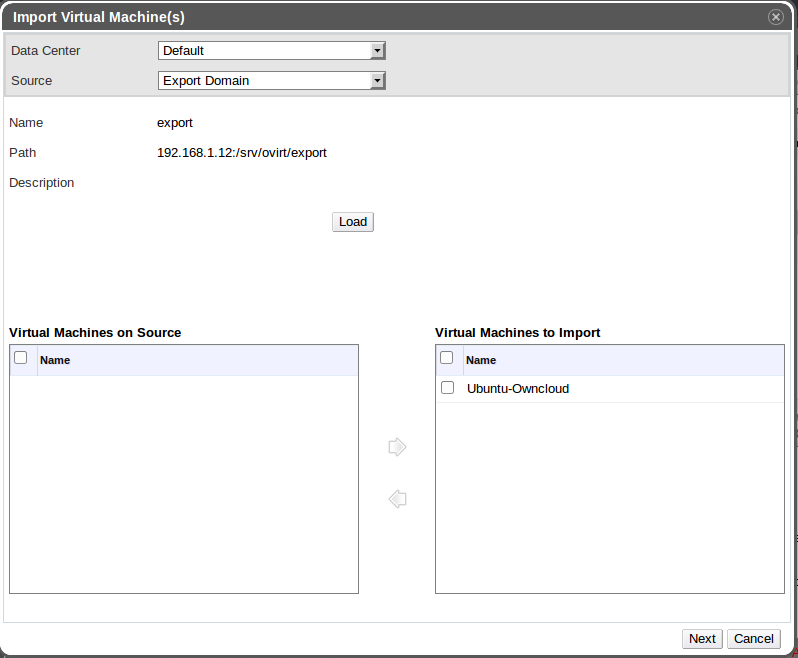
\includegraphics[scale=0.45]{ovirt_import1.png}
  \caption{\label{fig:import_start} Iniciando la importación}
\end{figure}

\begin{figure}[ht!]
  \centering
  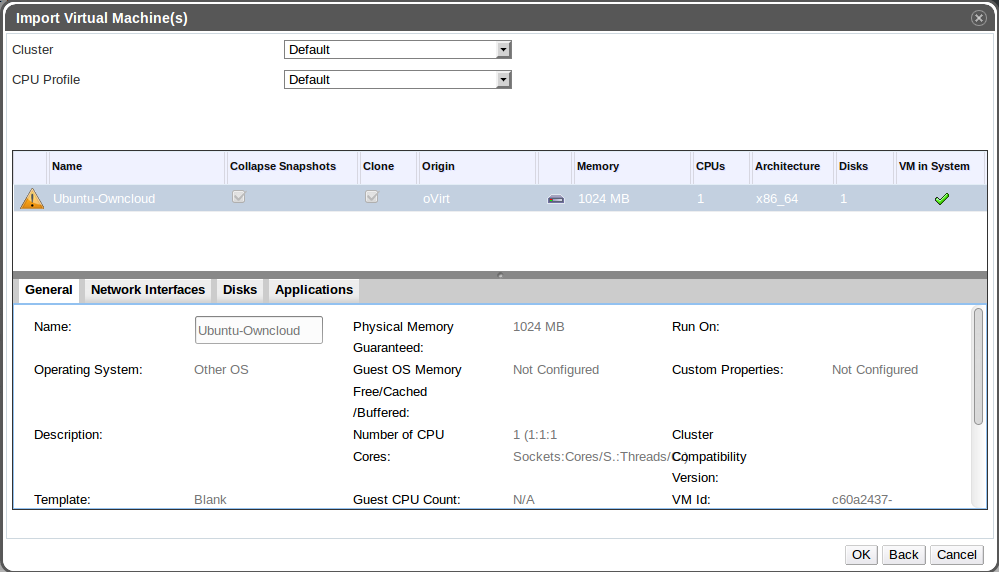
\includegraphics[scale=0.45]{ovirt-import2.png}
  \caption{\label{fig:import_start} Siguiendo la importación}
\end{figure}
\clearpage

\section{Clonando máquinas virtuales}
\label{sec:consola}

La clonación de máquinas virtuales en oVirt es probablemente la operación más sencilla a realizar. Simplemente debemos darle un nombre nuevo, y se generará una copia exacta de la máquina, configuración incluida.

\section{Migrando máquinas virtuales}
\label{sec:migración}

La migración de las máquinas virtuales permite mantener una máquina virtual en ejecución, mientras la carga de trabajo se traslada a otro host. Aunque en papel suena muy útil, en mis pruebas ha sido bastante \emph{hit or miss}(acierto o error). Una vez apretado el botón para iniciar la migración, aparecerá la siguiente pantalla:

\begin{figure}[ht!]
  \centering
  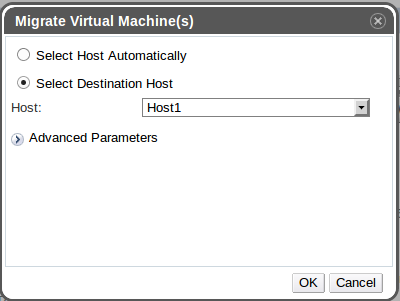
\includegraphics[scale=0.55]{Migration.png}
  \caption{\label{fig:migration_start} Iniciando la migración}
\end{figure}

Una vez seleccionado el host al cual queremos migrar, simplemente habrá que esperar. Si la migración ha funcionado, veremos como el campo Host del listado de máquinas virtuales habrá cambiado. Podemos ver cómo progresa la tarea en la parte de abajo de la web, en la sección Tasks:

\begin{figure}[ht!]
  \centering
  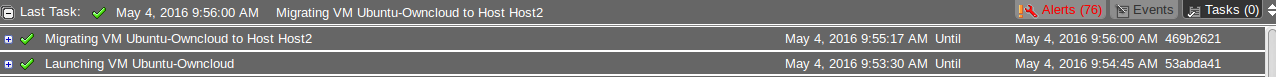
\includegraphics[scale=0.40]{migration_success.png}
  \caption{\label{fig:successful_migration} Migración exitosa}
\end{figure}

\section{Snapshots}
\label{sec:consola}

Una instantánea o \emph{snapshot} es el estado de una máquina virtual y sus discos en cualquier punto en el tiempo. Esto permite volver a un estado anterior si ocurre cualquier error que deje la máquina virtual inservible.

Para realizar un Snapshot, basta con darle a \textbf{Create Snapshot} en la barra de herramientas:

\begin{figure}[ht!]
  \centering
  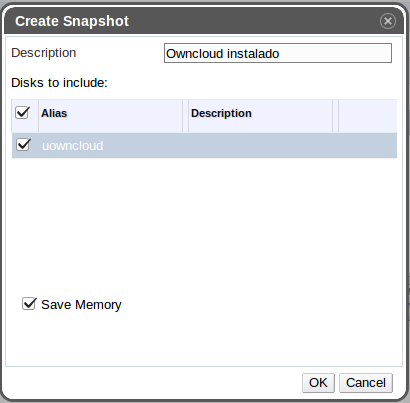
\includegraphics[scale=0.55]{snapshot.png}
  \caption{\label{fig:snapshot} Creación de snapshots}
\end{figure}

\begin{TMbulletin}{normal}{Nota}
  Si se usa almacenamiento NFS, tanto los discos virtuales, como los snapshots, son ficheros. Ésto quiere decir que las copias de seguridad pueden realizarse tranquilamente mediante scripts que copien los ficheros relevantes, y automatizarlos mediante \emph{crontab}.
\end{TMbulletin}

